%%% background to the research work
\chapter{Introduction} % at least 5 pages, not more than 10

%%%%%%%%%%%%%%%%%%%%%%%%%%%%%%%%%%%%%%%%%%%%%%%%%%%%%%%%%%%%%%%%%%%%%%%%%%%%%%%%
\section{Computer-aided Drug Discovery and Design}
  \subsection{Computational Methods}
    In the last decades, the development of new pharmaceuticals has been significantly boosted by the field of \textit{computer-aided drug discovery and design}. Computational methods allow to automate the exploration of a huge space of molecule configurations, with the goal of predicting which compounds would elicit desired biologic responses, and which others can be disregarded. According to these predictions, the molecules with the most therapeutic potential can be prioritized in further experimental stages, saving time and resources in the process of finding new benefitial drugs \cite{drug_discovery_2014}.

    Computational methods for drug discovery can be categorized in two main branches: \textit{ligand-based} (LBDD) and \textit{structure-based} (SBDD). Ligand-based methods focus only in the ligand and try to predict the behaviour of new molecules by taking as reference the activity of other known strucurally similar ligands. Structure based methods use information from the 3D structures of both ligand and target, and include approaches such as \textit{ligand docking}, \textit{molecular dynamics simulations} and \textit{pharmacophore modeling} \cite{drug_discovery_2014, structure_based_2019}.

  \subsection{Target Molecules and Binding Pockets}
    Although SBDD methods require the additional knowledge of the target structure (which is not trivial), they have been proven to be powerful and efficient methods in drug discovery \cite{structure_based_2019}. Consequently, the first basic step of SBDD methods is resolving the 3D structure of the therapeutically important \textbf{target molecule}, which traditionally refers to some protein of interest \cite{structure_based_2019}. However, this is not always the case, as in more recent years relevant RNA structures have also started to be considered as target molecules \cite{rna_targets_2022}.

    \begin{figure}[H]
      \centering
      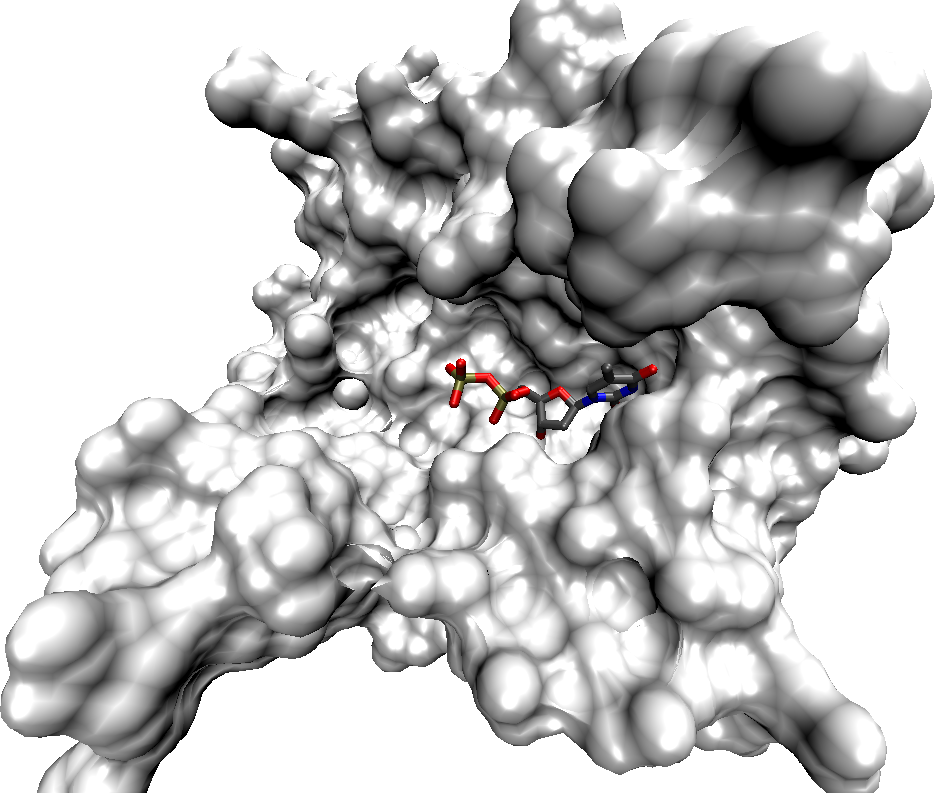
\includegraphics[width=0.5\textwidth]{figures/intro/pocket.png}
      \caption{\label{fig:intro/pocket} Ligand bound to the pocket of a protein (PDB:1h7l).}
    \end{figure}

    Once the structure of the target is well known, an appropriate \textbf{binding pocket} must be identified. This refers to a small cavity in the target where a ligand should bind to produce the desired effect (figure \ref{fig:intro/pocket}). Once this binding site is identified, different SBDD techniques can be performed, such as \textit{virtual screening}, \textit{de novo drug design}, \textit{molecular docking} and \textit{pharmacophore modeling}, among others \cite{drug_discovery_2014, structure_based_2019, pharmacophore_and_VS_2022}.

  \subsection{Virtual Screening and Pharmacophores}
    \textbf{Virtual screening} is a series of computational methods where a dataset of chemical compounds is reduced to only those with some chemical characteristics of interest, which generally means those with higher binding affinity to a given target pocket \cite{pharmacophore_and_VS_2022, virtual_screening_2019}. Given the immense chemical space of potential ligands, with curated databases consisting of millions of compounds, blindly performing virtual screening over whole datasets is often unpractical \cite{virtual_screening_2013}. This process can be however optimized by using \textit{pharmacophores} to reduce the search space to only those molecules that best satisfy some desired properties \cite{pharmacophore_and_VS_2022}.

    \textbf{Pharmacophore} models describe the spatial arrangement of steric and electronic features that allow ligands to optimally interact with their target binding sites \cite{pharmacophore_and_VS_2022, virtual_screening_2019, pharmacophore_modeling_2022, drug_discovery_2014}. The core idea behind pharmacophores is that ligands with common physicochemical properties and spatial arrangements should have a similar biological activity on the same target. The most relevant pharmacophoric features include \textit{positively and negatively charged groups}, \textit{aromatic groups}, \textit{hydrogen bond acceptors/donors}, \textit{hydrophobic areas}, \textit{exclusion volumes}, among others (figure \ref{fig:intro/pharmacophores}) \cite{pharmacophore_and_VS_2022, drug_discovery_2014}.

    \begin{figure}[H]
      \centering
      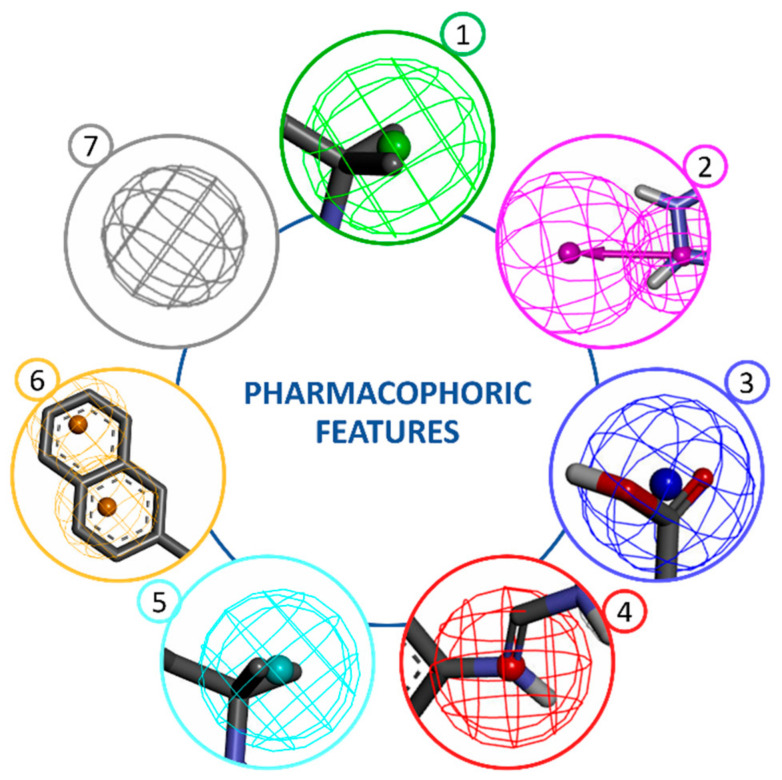
\includegraphics[width=0.5\textwidth]{figures/intro/pharmacophores.jpg}
      \caption{\label{fig:intro/pharmacophores} Summary of the main pharmacophoric features. 1) hydrogen bond acceptors, 2) hydrogen bond donors, 3) negatively charged, 4) positively charged, 5) hydrophobic, 6) aromatic, 7) exclusion volume. Adapted from \cite{pharmacophore_and_VS_2022}.}
    \end{figure}

    Pharmacophores can be modeled in either LBDD and SBDD pipelines. In the case of a structure-based approach, the pharmacophore can be obtained by different strategies. A completely target-based method can be employed, in which the pharmacophoric features are inferred by performing an analysis of the binding pocket's structure \cite{pharmacophore_and_VS_2022, virtual_screening_2019}.

    A more experimental approach involves molecular docking of different molecules from a ligand dataset, clustering the fragments with best affinity and extracting pharmacophore features from these clusters. Another straightforward and still effective strategy can be followed when experimental structures of target-ligand complexes are available. In this case, the pharmacophore features can be built based on this ligand, whose bioactive conformation is already known \cite{virtual_screening_2019}.


%%%%%%%%%%%%%%%%%%%%%%%%%%%%%%%%%%%%%%%%%%%%%%%%%%%%%%%%%%%%%%%%%%%%%%%%%%%%%%%%
\section{Protein and RNA Binding Sites}
  [TODO: How do ligands bind to pockets? physicochemical properties behind the pocket-ligand interactions in proteins and RNAs]

  \subsection{Hydrogen Bonds}
    [TODO]

  \subsection{Stacking}
    [TODO]

  \subsection{Electrostatics}
    [TODO]

  \subsection{Hydrophobicity}
    [TODO]

%%%%%%%%%%%%%%%%%%%%%%%%%%%%%%%%%%%%%%%%%%%%%%%%%%%%%%%%%%%%%%%%%%%%%%%%%%%%%%%%
\section{Molecular Visualization Software}
  [TODO: Usual approach of studying the pockets (ie description of the surfaces)]

  [TODO: Methods already employed for visualizing the physical properties described before (hbonds, stacking...)]

  \subsection{UnityMol}
    [TODO: Introduction to UnityMol]

%%%%%%%%%%%%%%%%%%%%%%%%%%%%%%%%%%%%%%%%%%%%%%%%%%%%%%%%%%%%%%%%%%%%%%%%%%%%%%%%
